% ============================================================================
% ICLR 2027 draft — S-LoRA (Squared LoRA)
%
% VA CHAM TEN: "S-LoRA" da bi dung boi Sheng et al., MLSys 2024
% ("S-LoRA: Serving Thousands of Concurrent LoRA Adapters") — cung linh vuc
% LoRA + LLM va duoc cite nhieu. Phai quyet dinh giu hay doi (SqLoRA /
% Sq-LoRA) TRUOC khi nop, khong de den luc camera-ready.
%
% PHAM VI: CHI Qwen2.5-1.5B / E2E NLG. Thi nghiem Llama/commonsense da duoc
% loai khoi paper (code va ket qua van con o finetune_commonsense.py va
% Downloads/ll/llama_cs2/). Vi da thu hep bang chung, MOI khang dinh trong
% file nay cung da duoc thu hep theo — dung noi rong hon pham vi da test.
%
% Moi con so deu tu run that, da kiem lai ngay 2026-09-02. Cho nao chua co
% du lieu thi \TODO{} — KHONG dien so vao roi chay sau.
% ============================================================================
\documentclass{article}
\usepackage{iclr2027_conference,times}
\usepackage{amsmath,amssymb,booktabs,graphicx,microtype,url,xcolor}

\newcommand{\TODO}[1]{\textcolor{red}{[TODO: #1]}}

\title{S-LoRA: Squared LoRA via Exact Row-Space Factorization\\
       for Parameter-Efficient Fine-Tuning}
\author{Hiep Nguyen}

\begin{document}
\maketitle

% ---------------------------------------------------------------- ABSTRACT
\begin{abstract}
Parameter-efficient fine-tuning adapts a frozen weight through an additive
low-rank correction whose cost scales with both of the weight's dimensions ---
wasteful precisely where modern architectures are most compressed, since
grouped-query attention leaves key and value projections with aspect ratios of
six in Qwen2.5-1.5B and seventy-one in Falcon-7B, so the adapter pays for a
long dimension carrying no matching capacity. Shrinking the adapted object is
the obvious remedy, but existing routes either train a zero-initialized delta,
leaving methods that exploit pretrained structure nothing to attach to, or
truncate to the leading spectral directions and surrender exactness. We propose
\textbf{S-LoRA} (Squared LoRA), which reparametrizes the layer instead of
adding to it: an exact factorization splits each non-square weight into a
frozen rectangular factor and a square factor that retains its pretrained
values, and adaptation is applied to the square factor alone, confining the
update to the row space of the pretrained weight. The reparametrization is
lossless in both output and parameter count, folds back into a single matrix
at deployment, and --- because the adapted matrix is square --- makes any
dimension-scaled adapter cheaper by a factor set by the weight's aspect ratio.
Fine-tuning Qwen2.5-1.5B on E2E NLG through the key and value projections
alone, S-LoRA saturates at $0.057$M trainable parameters and $65.2$ BLEU ---
above the $64.3$ that unconstrained training of those same matrices reaches
with $22.0$M, and unmatched by LoRA until $0.803$M --- and leads LoRA by
$2.75$, $1.21$ and $0.72$ BLEU ($4.0\sigma$, $2.7\sigma$, $1.3\sigma$) at
matched budgets, though the margin vanishes above $0.25$M and reverses at rank
one. Within this one model and task family, constraining updates to the
pretrained row space is a favorable trade wherever the budget is small; and
because the trainable object stays a pretrained square matrix, S-LoRA composes
with the adapter family instead of competing with it.
\end{abstract}

% ------------------------------------------------------------ INTRODUCTION
\section{Introduction}

Adapting a pretrained language model to a downstream task by updating all of
its weights is rarely practical, and the field has converged on a common
answer: keep $W_0$ frozen and learn a small additive correction. LoRA
\citep{hu2022lora} parametrizes that correction as a rank-$r$ product $BA$;
the many variants that followed change how $B$ and $A$ are initialized,
scaled, allocated, or shared, but they all inherit the same additive skeleton
$W_0 + \Delta W$. The cost of every such adapter is $O(r(n+m))$ --- it scales
with \emph{both} dimensions of the weight it adapts.

That scaling is wasteful for lopsided matrices, and modern architectures are
full of them. Grouped-query attention \citep{ainslie2023gqa} deliberately
compresses the key and value projections: in Qwen2.5-1.5B they map $1536$
inputs to $256$ outputs, an aspect ratio of six; in Falcon-7B the ratio
reaches $71$. An adapter that pays for the long dimension is paying for
capacity the layer itself does not have. The obvious remedy --- adapt a
smaller object --- runs into a second problem: the small object must still
carry pretrained information, or methods that exploit pretrained structure
(magnitude--direction decomposition \citep{liu2024dora}, principal-component
initialization \citep{meng2024pissa}) have nothing to attach to. Prior work
that builds adapters from the rows and columns of $W_0$ itself
\citep{wang2024pmss,pica2025} comes close, but the trainable object is still a
zero-initialized delta.

We take a different route: replace the layer with an exact factorization
instead of adding to it. Column-pivoted QR selects $k = \min(n,m)$ columns of
$W$ that are as well-conditioned as the greedy criterion can find, and the
remaining columns are written exactly in terms of them. The identity block
costs nothing to store or apply --- it is an index selection, not a matmul ---
so the reparametrized layer has the same parameter count and the same FLOP
count as the original, and folds back into a single matrix at deployment. What
changes is what is adaptable: the trainable object is now a square
$k \times k$ matrix that still holds pretrained values, so the entire adapter
toolbox applies to it, each tool becoming cheaper by $(1+a)/2$.

Constraining $\Delta W$ this way is not free, and its price depends on the
budget it is spent under. On Qwen2.5-1.5B fine-tuned for E2E NLG with only the
key and value projections adapted, the constraint behaves as a regularizer in
the low-budget regime: quality saturates at rank two --- $0.057$M trainable
parameters, under $0.004\%$ of the model --- and at that point already exceeds
what unconstrained training of those same two matrices achieves with $384\times$
more parameters. Against LoRA at matched budget the lead is $2.75$ BLEU near
$0.1$M and $1.21$ near $0.2$M, but it narrows to $0.72$ by $0.4$M and inverts
at rank one, where the constrained model has too few directions to work with.
The method is a low-budget instrument, not a universal replacement, and we
present it as one.

\paragraph{Contributions.}
\begin{itemize}
  \item An exact, parameter-preserving reparametrization of non-square weights
        via interpolative decomposition, with a closed-form cost advantage
        $(1+a)/2$ for dimension-dependent adapters and $a$ for full
        fine-tuning.
  \item An analysis showing that adapting the square factor is equivalent to
        preconditioned gradient descent on the original weight,
        $\Delta W = -\eta (\partial L/\partial W)(P^\top P)$, with the
        preconditioner reducing to an orthogonal projector exactly when the
        basis is orthonormal.
  \item A controlled comparison against LoRA, an unconstrained upper bound,
        and the zero-shot floor across five parameter budgets spanning
        $16\times$, with two to three seeds per configuration.
\end{itemize}

% ------------------------------------------------------------------- SKELETON
\section{Related Work}
\TODO{Muc rui ro nhat cua ca paper. Ba nhom, phai xu ly thang, khong duoc ne.}
\paragraph{Skeleton and CUR-based adapters.} PMSS \citep{wang2024pmss} dung
dung pivoted QR de chon hang/cot cua $W_0$ va cung phat bieu rang buoc khong
gian con. Khac biet phai neu ro: mot phia thay vi hai phia; nhan thay vi cong;
bao toan tham so.
\paragraph{Spectral initialization.} PiCa \citep{pica2025}, LoRA-XS, PiSSA,
MiLoRA.
\paragraph{Structural reparametrization.} ExpandNets, RepVGG, va
SVD-restructuring trong nhan dang tieng noi (2013--2014).

\section{Method}

\subsection{Notation}
A linear layer maps $x\in\mathbb{R}^{m}$ to $y=W_0x$ with $W_0\in\mathbb{R}^{n\times m}$
frozen and $n\neq m$. Write
\[
  k=\min(n,m),\qquad a=\frac{\max(n,m)}{k}\ \ge 1 ,
\]
so $W_0$ holds $nm=ak^2$ entries, and LoRA's correction
$\Delta W=\tfrac{\alpha}{r}BA$, with $B\in\mathbb{R}^{n\times r}$ and
$A\in\mathbb{R}^{r\times m}$, costs $r(n+m)=rk(1+a)$ parameters per layer.
Every quantity below is per layer; $\langle\cdot,\cdot\rangle$ is the Frobenius
inner product; $[\,A\mid B\,]$ and $[\,A\,;B\,]$ denote horizontal and vertical
concatenation.

\begin{figure}[t]
\centering
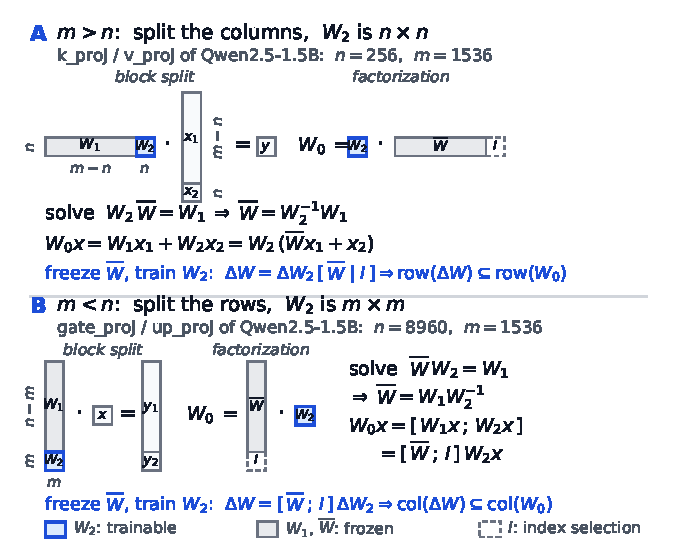
\includegraphics[width=\textwidth]{fig_orientations.pdf}
\caption{Splitting a non-square weight. \textbf{(A)} When $m>n$ the columns
split, $W_0=[\,W_1\mid W_2\,]$ with $W_2$ square, and solving
$W_2\overline{W}=W_1$ gives $W_0=W_2[\,\overline{W}\mid I\,]$: the input is
mixed \emph{before} the square factor, so the update stays in
$\operatorname{row}(W_0)$. \textbf{(B)} When $m<n$ the rows split,
$W_0=[\,W_1\,;W_2\,]$, and solving $\overline{W}W_2=W_1$ gives
$W_0=[\,\overline{W}\,;I\,]W_2$: the output is expanded \emph{after} it, so the
update stays in $\operatorname{col}(W_0)$. Blue marks $W_2$, the only object
adaptation touches and one that still holds pretrained values; grey marks the
frozen blocks; the dashed identity is an index selection costing neither
parameters nor FLOPs. Rectangles are drawn to the true aspect ratios of the
layers named. Regenerate with \texttt{python paper/fig\_orientations.py}.}
\label{fig:orient}
\end{figure}

\subsection{Splitting a non-square weight}
\label{sec:split}
\paragraph{More inputs than outputs ($m>n$, $k=n$).}
Split the columns of the weight, and the entries of $x$ conformally
(Figure~\ref{fig:orient}A):
\[
  W_0=[\,W_1 \mid W_2\,],\qquad
  W_1\in\mathbb{R}^{n\times(m-n)},\quad W_2\in\mathbb{R}^{n\times n},
  \qquad x=[\,x_1\,;x_2\,].
\]
Whenever the square block $W_2$ is nonsingular, the rectangular block is
determined by it: solving
\begin{equation}
  W_2\,\overline{W}=W_1
  \qquad\Longleftrightarrow\qquad
  \overline{W}=W_2^{-1}W_1\in\mathbb{R}^{n\times(m-n)}
  \label{eq:solve-wide}
\end{equation}
rewrites the layer with no approximation whatsoever,
\begin{equation}
  W_0x \;=\; W_1x_1+W_2x_2 \;=\; W_2\bigl(\overline{W}x_1+x_2\bigr),
  \qquad\text{that is}\qquad
  W_0 \;=\; W_2\,[\,\overline{W}\mid I_n\,].
  \label{eq:wide}
\end{equation}

\paragraph{More outputs than inputs ($n>m$, $k=m$).}
Split the rows instead, and $y$ conformally (Figure~\ref{fig:orient}B):
\[
  W_0=[\,W_1\,;W_2\,],\qquad
  W_1\in\mathbb{R}^{(n-m)\times m},\quad W_2\in\mathbb{R}^{m\times m},
  \qquad y=[\,y_1\,;y_2\,].
\]
Now the square block multiplies from the right, so the solve transposes:
\begin{equation}
  \overline{W}\,W_2=W_1
  \qquad\Longleftrightarrow\qquad
  \overline{W}=W_1W_2^{-1}\in\mathbb{R}^{(n-m)\times m},
  \label{eq:solve-tall}
\end{equation}
and
\begin{equation}
  W_0x \;=\; [\,W_1x\,;W_2x\,] \;=\; [\,\overline{W}W_2x\,;W_2x\,]
        \;=\; [\,\overline{W}\,;I_m\,]\,W_2x,
  \qquad\text{that is}\qquad
  W_0 \;=\; [\,\overline{W}\,;I_m\,]\,W_2 .
  \label{eq:tall}
\end{equation}
In both cases the layer has been rewritten as a square factor $W_2$ carrying
pretrained values, multiplied by a rectangular factor that contains an identity
block; adaptation is applied to $W_2$ and $\overline{W}$ is frozen. Writing
\begin{equation}
  P=[\,\overline{W}\mid I_n\,]\ \ (m>n),
  \qquad
  P=[\,\overline{W}\,;I_m\,]\ \ (n>m),
  \qquad
  W_0=W_2P \ \text{ or } \ W_0=PW_2,
  \label{eq:P}
\end{equation}
lets the two cases be treated together below.

\paragraph{Which block is the square one.}
Equations~\eqref{eq:wide} and~\eqref{eq:tall} hold for any choice of $n$
columns (resp.\ $m$ rows) as $W_2$, but not equally well: taking the last ones
leaves $W_2$ badly conditioned and inflates $\|\overline{W}\|$, which costs
accuracy in low precision. We choose them by column-pivoted QR,
$W_0\Pi=Q\,[\,R_{11}\mid R_{12}\,]$, which additionally makes the solve cheap.
With $W_2=QR_{11}$ the selected block and $W_1=QR_{12}$ the rest,
\begin{equation}
  \overline{W}=W_2^{-1}W_1=(QR_{11})^{-1}(QR_{12})=R_{11}^{-1}R_{12}:
  \label{eq:qcancel}
\end{equation}
the orthogonal factor cancels, so $\overline{W}$ costs one triangular solve,
$Q$ is never formed and $W_2$ never inverted. The relative residual of the
resulting identity is $6.6\times 10^{-15}$ in float64.
\TODO{xac nhan con so nay do tren Qwen2.5-1.5B hay GPT-2 M}
Pivoting only permutes which coordinates carry the identity, so~\eqref{eq:P}
becomes $P=[\,\overline{W}\mid I_n\,]\Pi^{\top}$ and, in the row case,
$P=\tilde{\Pi}^{\top}[\,\overline{W}\,;I_m\,]$.

\paragraph{Orthonormal variant.}
Replacing the pivoted-QR basis by the thin SVD $W_0=U\Sigma V^{\top}$ gives the
same two forms --- $W_2=U\Sigma,\ P=V^{\top}$ when $m>n$, and
$P=U,\ W_2=\Sigma V^{\top}$ when $n>m$ --- now with $P$ orthonormal. The two
bases span the same solution set and carry the same number of trainable
parameters; they differ in conditioning, $\kappa(P)=1$ against
$\kappa([\,\overline{W}\mid I\,])$, and in storage
(Section~\ref{sec:acct}).

\paragraph{Cost of the rewritten layer.}
The identity block is an index gather, not a matmul, so evaluating
$W_2(\overline{W}x_1+x_2)$ costs $n(m-n)+n^2=nm$ multiply--accumulates ---
exactly the cost of $W_0x$ --- and~\eqref{eq:tall} is the same count by
symmetry.

\subsection{The constraint this imposes}
Adaptation touches $W_2$ only, holding $\overline{W}$ fixed. Substituting
$W_2\mapsto W_2+\Delta W_2$ into~\eqref{eq:wide} and~\eqref{eq:tall} gives
\begin{equation}
  \Delta W=\Delta W_2\,[\,\overline{W}\mid I\,]
  \;\Longrightarrow\;
  \operatorname{row}(\Delta W)\subseteq\operatorname{row}(W_0),
  \qquad
  \Delta W=[\,\overline{W}\,;I\,]\,\Delta W_2
  \;\Longrightarrow\;
  \operatorname{col}(\Delta W)\subseteq\operatorname{col}(W_0),
  \label{eq:constraint}
\end{equation}
the row-space identity following from
$\operatorname{row}(P)=\operatorname{row}(W_0)$ whenever $W_2$ is nonsingular.
The containment is exact and holds for \emph{every} $\Delta W_2$; it is
therefore a property of the parametrization, not of the optimizer.

The constraint is far from vacuous. It confines $\Delta W$ to a $k$-dimensional
subspace of a $\max(n,m)$-dimensional ambient space, so an update with no
alignment to $W_0$ would keep, in expectation, only a $1/a$ fraction of its
squared Frobenius norm. The quantity the constraint must beat is accordingly
$\rho=\|\Delta W\,VV^{\top}\|_F^2/\|\Delta W\|_F^2$ measured on an unconstrained
fine-tune, against a chance level of $1/a$ ($0.167$ at $a=6$).
\TODO{do rho tren target-ft Qwen2.5-1.5B}

Both cases are implemented, but every experiment in this paper uses the first
(\texttt{k\_proj} and \texttt{v\_proj} of Qwen2.5-1.5B, $a=6$); we make no
empirical claim about the second.

\subsection{Which object is trained}
Two variants sit on top of the same split. \emph{(i) Direct:} $W_2$ is itself
the trainable parameter, initialized at its pretrained value --- $k^2$
parameters per layer, and no zero-initialized delta anywhere in the layer.
\emph{(ii) Adapter-on-square:} $W_2$ is frozen and
$\Delta W_2=\tfrac{\alpha}{r}BA$ with $B\in\mathbb{R}^{k\times r}$,
$A\in\mathbb{R}^{r\times k}$ and $B$ zero-initialized --- $2rk$ parameters, and
the layer reduces to the pretrained one at initialization. Composing (ii)
with~\eqref{eq:wide} states what S-LoRA is in LoRA's own terms:
\begin{equation}
  \Delta W \;=\; \tfrac{\alpha}{r}\,B\,(A P),
  \label{eq:restricted-lora}
\end{equation}
a rank-$r$ update whose down-projection $AP\in\mathbb{R}^{r\times m}$ is
trainable but confined to $\operatorname{row}(W_0)$. S-LoRA at rank $r$ is thus
\emph{restricted} LoRA at rank $r$, and the question it poses is whether a
down-projection drawn from the pretrained row space beats an unconstrained one
or a frozen random one --- which makes LoRA-FA the sharpest missing baseline.
\TODO{them LoRA-FA vao Related Work va bang ket qua}

\subsection{Parameter and FLOP accounting}
\label{sec:acct}
The pivoted-QR form stores $W_2$ ($k^2$ floats) and $\overline{W}$
($k(\max(n,m)-k)$ floats), totalling $k\max(n,m)=nm$ floats plus $\max(n,m)$
integer indices: byte-for-byte the original weight. The SVD form stores $P$
densely instead of the identity block and costs an extra $k^2$ per layer. In
both cases~\eqref{eq:wide} and~\eqref{eq:tall} fold back into a single
$n\times m$ matrix after training, so deployment is unchanged.

What shrinks is the object an adapter attaches to: $k\times k$ instead of
$n\times m$. For any adapter whose parameter count scales as $c\,r(n+m)$, the
cost drops from $c\,rk(1+a)$ to $2c\,rk$, a saving of
\begin{equation}
  \frac{\text{cost on }W_0}{\text{cost on }W_2}\;=\;\frac{1+a}{2},
  \label{eq:saving}
\end{equation}
and full fine-tuning drops from $ak^2$ to $k^2$, a saving of $a$
(Table~\ref{tab:acct}). The saving is a property of the adapter's cost model
rather than of our method, and it is worth stating plainly where it does
\emph{not} apply: adapters whose parameter count is independent of the layer's
dimensions --- LoRA-XS, which trains an $r\times r$ core, and PMSS
\citep{wang2024pmss} --- gain nothing from a smaller adapted matrix, and
$(1+a)/2$ must not be quoted against them.

\begin{table}[t]\centering
\caption{Trainable parameters per layer before and after the rewrite, with
$k=\min(n,m)$ and $a=\max(n,m)/k$. The last group is dimension-independent and
gains nothing.}
\label{tab:acct}
\begin{tabular}{lrrl}
\toprule
Adapted with & on $W_0$ & on $W_2$ & saving \\
\midrule
full fine-tuning  & $ak^2$              & $k^2$    & $a$ \\
LoRA rank $r$     & $rk(1+a)$           & $2rk$    & $(1+a)/2$ \\
DoRA rank $r$     & $rk(1+a)+\max(n,m)$ & $2rk+k$  & $(1+a)/2$ asymptotically \\
VeRA rank $r$     & $r+n$               & $r+k$    & orientation-dependent \\
\midrule
LoRA-XS rank $r$  & $r^2$               & $r^2$    & $1$ \\
PMSS rank $r$     & $r^2$               & $r^2$    & $1$ \\
\bottomrule
\end{tabular}
\end{table}

\subsection{What the constraint does to the gradient}
Let $G=\partial L/\partial W$ be the gradient with respect to the original
weight. For $m>n$ trained through variant (i), $W=W_2P$ gives
$\langle G,dW\rangle=\langle G,dW_2\,P\rangle=\langle GP^{\top},dW_2\rangle$, so
$\partial L/\partial W_2=GP^{\top}$, and one gradient step
$W_2\leftarrow W_2-\eta\,GP^{\top}$ induces
\begin{equation}
  \Delta W \;=\; \Delta W_2\,P \;=\; -\eta\,\frac{\partial L}{\partial W}\,\bigl(P^{\top}P\bigr).
  \label{eq:precond}
\end{equation}
Training the square factor is therefore \emph{exactly} preconditioned gradient
descent on the original weight, with a fixed symmetric positive-semidefinite
preconditioner $M=P^{\top}P\in\mathbb{R}^{m\times m}$ of rank $k$ and range
$\operatorname{row}(W_0)$. The $n>m$ case is the mirror image,
$\Delta W=-\eta\,(PP^{\top})\,\partial L/\partial W$, a left preconditioner with
range $\operatorname{col}(W_0)$.

The basis decides what $M$ does inside that range. For the orthonormal basis
$P=V^{\top}$,
\[
  M=VV^{\top},\qquad M^2=M,
\]
a pure orthogonal projector: the step is the unconstrained step projected onto
$\operatorname{row}(W_0)$, with no rescaling. For the pivoted-QR basis
$P=[\,\overline{W}\mid I\,]\Pi^{\top}$,
\[
  M=\Pi\begin{bmatrix}
        \overline{W}^{\top}\overline{W} & \overline{W}^{\top}\\
        \overline{W} & I
      \end{bmatrix}\Pi^{\top},
  \qquad M^2\neq M,
\]
which projects onto the same subspace but also rescales it anisotropically, the
distortion governed by $\kappa(P)$. This is why the two bases --- despite
spanning an identical solution set and carrying identical parameter counts ---
need not reach the same optimum, and it is what the basis ablation isolates.

Two caveats. First,~\eqref{eq:precond} is stated for plain gradient descent;
under Adam the containment~\eqref{eq:constraint} still holds exactly, since it
holds for arbitrary $\Delta W_2$, but the preconditioner reading is only a
first-order description of the trajectory. Second, under variant (ii) the same
containment holds with $\Delta W_2$ supplied by the adapter, so
\eqref{eq:constraint} and~\eqref{eq:restricted-lora} are unaffected by the
choice of optimizer.

\section{Experimental Setup}
\TODO{Mot model, mot benchmark — noi thang pham vi ngay o day, khong don
      xuong limitations. Sieu tham so theo paper LoRA. Tai lap bit-exact.
      Ghim phien ban thu vien.}

\section{Results}
\TODO{Hinh Pareto 5 rank x 2 phuong phap + hai duong ngang target-ft
      (22.03M, 64.26) va zero-shot (33.12). Nhan manh so sanh CUNG NGAN SACH;
      giai thich vi sao so cung rank la sai (LoRA duoc 3.5x tham so o do).}

% So lieu da kiem lai 2026-09-02, da loai cac run tu code cu (thieu epochs_run).
\begin{table}[t]\centering
\caption{Qwen2.5-1.5B, \texttt{k\_proj}+\texttt{v\_proj} ($a{=}6$), E2E NLG.}
\begin{tabular}{lrrrrr}
\toprule
Method & $r$ & Params & BLEU & sd & $n$ \\
\midrule
S-LoRA    &1  & 0.029M & 62.45 & 0.33 & 2 \\
S-LoRA    &2  & 0.057M & 65.22 & 0.22 & 2 \\
S-LoRA    &4  & 0.115M & \textbf{65.53} & 0.14 & 3 \\
S-LoRA    &8  & 0.229M & 65.45 & 0.38 & 3 \\
S-LoRA    &16 & 0.459M & 65.70 & 0.38 & 2 \\
\midrule
LoRA      & 1  & 0.100M & 62.78 & 0.97 & 2 \\
LoRA      & 2  & 0.201M & 64.24 & 0.50 & 2 \\
LoRA      & 4  & 0.401M & 64.98 & 0.70 & 3 \\
LoRA      & 8  & 0.803M & 65.61 & 0.07 & 3 \\
LoRA      & 16 & 1.606M & 65.75 & 0.06 & 2 \\
\midrule
target-ft & -- & 22.034M & 64.26 & -- & 1 \\
zero-shot & -- & 0 & 33.12 & -- & 1 \\
\bottomrule
\end{tabular}
\end{table}

\section{Regime Boundaries}
Two limits fall out of the same sweep, and we state them as findings rather
than caveats. First, the advantage is confined to the low-budget regime: it
is $2.75$ BLEU at $0.1$M and $1.21$ at $0.2$M, but only $0.72$ ($1.3\sigma$)
at $0.4$M, and both methods converge to roughly $65.7$ thereafter. Second,
at rank one the constrained model \emph{loses} to LoRA, $62.45$ against
$62.78$: with a single direction the row-space restriction removes capacity
faster than it removes noise.
\TODO{Them mot doan giai thich co che cho ca hai bien.}

\section{Ablations}
\TODO{Chua chay cai nao. Uu tien: (1) PMSS cung duong Pareto — quan trong
      nhat; (2) co so SVD vs colperm — cung khong gian nghiem nen chenh lech
      co lap dung hieu ung preconditioning; (3) dong bang $W_2$ train $X$ de
      chung minh loi ich den tu rang buoc chu khong tu viec co mot phep
      phan ra.}

\section{Limitations}
Our evidence comes from a single model and a single task family; we make no
claim about transfer to other architectures or to tasks of a different
character. The method touches only $1.4\%$ of the model's weights: square
matrices admit no such factorization, so the query and output projections ---
and every attention matrix in a model without grouped-query attention --- fall
outside its scope. The advantage exists only at low budget and reverses at
rank one, as Section~7 reports. Finally, we do not yet compare against
skeleton-based adapters such as PMSS, which select from $W_0$ by the same
pivoted-QR criterion; establishing the empirical gap to that family is the
most important remaining experiment.

\bibliographystyle{iclr2027_conference}
\bibliography{refs}
\end{document}
